\documentclass[11pt,letterpaper]{article}
\usepackage[margin=1.0in]{geometry}
\usepackage{amssymb,amsmath,enumerate,mathtools}
\usepackage{graphics,graphicx}
\usepackage{framed, listings}

\lstset{
    language=Verilog,                            % sets the language for the code
    basicstyle=\scriptsize\ttfamily,       % for the actual code
    morekeywords={assign, logic, module, endmodule},  % adds keywords
    deletekeywords={if, do, for},               % removes keywords
    keywordstyle=\bfseries\textbf,                % for keywords
    commentstyle=\scriptsize\ttfamily\emph,     % for comments 
    showstringspaces=false                 % prevents underscores from appearing in output
}

\newcommand{\header}{\noindent\textbf}

\begin{document}
\begin{flushright}
Andrew Scott\\
E155\\
Lab 4\\
October 5, 2015
\end{flushright}

\begin{center}
Lab 4: Life of Pi
\end{center}

\header{Assembly Code}\\
\lstinputlisting{lab4_as.s}

\pagebreak

\header{Testing}\\
To test my sorting algorithm, I used three separate tests (by separate tests I am referring to the input array of unsorted bytes). I started with an array that had no particular order, but did have one number that repeated. This test was to ensure that the algorithm was generally working, given a random input, and that it could handle duplicates fine. Before running the algorithm, the array appeared as follows:\\
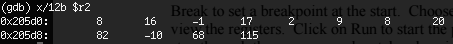
\includegraphics[scale=1.0]{test1Before}\\
After running the algorithm, the array was properly sorted, including the repeating 8 showing up next to itself as it was supposed to:\\
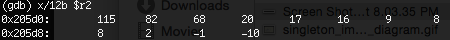
\includegraphics[scale=1.0]{test1After}\\\\
The second test I ran was with an array of bytes that was in completely reverse order. This would ensure that the algorithm was considering every element of the array when doing the sorting and not skipping over any of them. Before running the algorithm, the array appeared as follows:\\
\includegraphics[scale=1.0]{test2Before}\\
After running the algorithm, the array was completely reversed and thus sorted:\\
\includegraphics[scale=1.0]{test2After}\\\\
Finally, I ran a test on an already sorted array to ensure that the algorithm would not make any moves when it was not necessary to do so. Before running the algorithm, the array appeared as follows:\\
\includegraphics[scale=1.0]{test3Before}\\
After running the algorithm, the array was unchanged:\\
\includegraphics[scale=1.0]{test3After}\\\\\\

\header{Time}\\
I spent approximately 7 hours on this lab.
\end{document}

